\documentclass[a4paper]{ctexrep}

\usepackage{tikz}
\usepackage[version=4]{mhchem}
\usepackage{graphicx}
\usepackage{float}
\usepackage{xcolor}
\usepackage{mathtools}
\usepackage{booktabs}
\usepackage{chemfig}

\newcommand{\mol}{\mathrm{mol}}
\renewcommand{\d}{\mathrm{d}}


\title{结构化学B -- 那永}
\author{Y.C. Long}

% 考试要考的:
% 线性变分法,选定临界波函数 -> c1 c2 相同,想法。
% Huckel轨道法处理烯丙基
% 一维势箱,共轭体系能量高低
% 等性杂化
% 前线轨道,解释反应难易
% 光谱,算S, L
% 同核的分子轨道,N2,O2
% 核外电子排布,24 29,解释稳定性的问题(第二章)

% 考试不考的:
% 解薛定谔方程,绝对不会考
% 能级排序,选律不考
% 不等性杂化的推导
% 分子轨道理论里面异核的不看,只考同核的
% 分子轨道对称守恒,不考(前线轨道)
\begin{document}
\maketitle
\tableofcontents

\chapter{绪论}
\section{发展历史与研究内容}

用量子力学原理研究院子结构,化学键理论,分子结构,各种光谱和电子能谱(核磁的位置、红外吸收峰的位置),化学反应理论。

量化计算:各种无机有机分子间作用力,超分子,生物大分子,纳米材料的结构与性能关系的科学。

\section{学习目的和意义}

结构化学是四大化学的基础。

\begin{enumerate}
    \item 建立物质结构观点,更深层次了解物质结构及其反应本质
    \item 增强物质结构的意识
\end{enumerate}

物质结构基础 $\Rightarrow$ 量子化学 $\Rightarrow$ 量化计算(预测、模拟)

\chapter{量子力学基础}

三个著名的实验用经典力学解释不了,才有了量子力学的提出。这三个实验主要是:黑体辐射、光电效应、氢原子光谱。

\section{微观粒子的波粒二象性}

\subsection{光的波粒二象性}

\[
    h = 6.63 \times 10^{-34} \ \mathrm{m^2 kg / s}  
\]

\[
    p = mc = \frac{h}{\lambda} 
\]

\subsection{德布罗意波}

\[
    p = mc = \frac{h}{\lambda} 
\]

\subsubsection{电子的衍射实验}

1927年,美国科学家戴维逊--电子衍射实验。用电子射线发生器通过金属箔。

\subsection{不确定性关系}

有一些成对的可观测量,要同时测定他们的任意精确值是不可能的。

\[
    \Delta x \cdot \Delta p_x \geq h  
\]

\[
    \Delta y \cdot \Delta p_y \geq h  
\]

\section{量子力学的基本假设}

\subsection{波函数与几率}

\textit{假设一:微观粒子的运动状态可以用波函数来表示。}

含时波函数$\psi(x, y, z, t)$,定态波函数$\psi(x, y, z)$。用复值平面波来代表电子的运动状态。

\[
    p = |\psi|^2 \times V   
\]

波函数没有物理意义,$|\psi|^2$有物理意义,代表几率密度。在空间内电子的运动规律是其几率密度。

\subsubsection{波函数的重要性质}

$c\psi$与$\psi$描述同一状态。波函数前乘以一个系数,描述的状态不发生改变。

\subsection{力学量与算符}

算符就是表示运算过程中的符号。$\sqrt{}$ , $\frac{\mathrm{d}}{\mathrm{d}x}$,$\frac{\partial}{\partial x}$, $\frac{\partial^2}{\partial x^2}$

\[\hat{F}\psi = F \times \psi \]

\subsubsection{动量算符}

\[\hat{p} = \frac{h}{2 \pi i} \frac{\partial}{\partial x}\]

\textbf{举例:}

设

\[\psi = e^{ax}, \hat{F}\psi = \frac{\d \psi}{\d x} \]

\[
    \psi(x) = Ae^{\left(\frac{-2\pi i}{\hbar}\right)Et} e^{\frac{i}{\hbar}5x}
\]

\[
    \hat{p} \psi = 5 \times \psi   
\]

\[
    p_x = 5  
\]

\subsubsection{动能算符}

量子力学中,动能和动量的关系依然不变:

\[
    T = \frac{p^2}{2m}  
\]

\begin{align*}
    \Rightarrow \hat{T}_x \psi &= \frac{p^2}{2m} \psi  \\
    &= \frac{1}{2m}(p \cdot p \cdot psi) \\ 
    &= \frac{1}{2m} \left[\hat{p} \left( p \psi \right) \right] \left(
        \psi ' = p \cdot \psi
     \right) \\ 
    &= \frac{1}{2m} \left[ \hat{p} \cdot \left(
        \hat{p} \psi
     \right) \right] \\
    &= \frac{1}{2m} \frac{\d}{\d x} \left( \frac{\d \psi}{\d x} \right) \left( -i \hbar \cdot i \hbar \right) \\
    &= - \frac{\hbar^2}{2m} \frac{\d ^2}{\d x^2}
\end{align*}

\subsubsection{坐标算符和势能算符}

\[
    \hat{x} = x \cdot  
\]

\[
    \hat{x} \psi = x \cdot \psi  
\]

\[
    \hat{V} = V \cdot   
\]

\[
    \hat{V} \psi = V \cdot \psi  
\]


\subsubsection{哈密顿算符和总能量}

\[
    E_{\mbox{总}} = T + V  
\]

\subsection{本征值和本征方程}

如果按照算符作用到波函数,所求的动量在常数方向上具有本征值。如果算出来的东西是一个不确定量,那么这个算符就没有本征值。

\subsection{薛定谔方程(假设三)}

\[
    \hat{H} \psi = E \psi  
\]

\subsubsection{波函数的合格条件}

\begin{enumerate}
    \item 单值,保证空间几率密度的唯一化
    \item 二阶可导,否则方程无解
    \item 平方可积(归一化)
\end{enumerate}

\[
    \int \psi^{*} \cdot \psi d\tau = 1  
\]

或

\[
    \int \psi^{*} \cdot \psi d\tau = \mathrm{C} 
\]

归一化条件

\[
    \psi' = \frac{1}{\sqrt{k}} \cdot \psi  
\]

\subsection{平均值(假设四)}

\[
    \hat{x} \cdot \psi = x \cdot \psi  
\]

这种函数求不出本征值,可以考虑求平均值

\[
    \bar{F} = \frac{\int \psi^* \hat{F} \psi \d \tau}{\int \psi^* \psi \d \tau}
\]

\subsubsection{态叠加原理}

\[
    \psi = \sum_{i=1}^n c_i \psi_i
\]

系数对概率的贡献是平方关系。


\subsubsection{正交性}

两个状态间不影响,其积分为0。

\[
   \int c_ic_j \psi_i \psi_j d\tau = 0
\]

\[
   A = \frac{\int (c_1 \psi_x + c_2 \psi_y + c_3 \psi_z) \hat{F} (c_1 \psi_x^* + c_2 \psi_y^* + c_3 \psi_z^*)}{k} 
\]

如果$\hat{F}$有本征值,其本征值为$F$,则

\[
    A = \frac{\sum\limits_{i=1}^n |c_i|^2 F }{ \sum\limits_{i=1}^n |c_i|^2 } 
\] 


\subsubsection{泡利不相容原理}

描述多电子体系的完全波函数,交换其中任意两个电子的完全坐标,波函数是反对称的。

电子必须旋转720度,才能恢复到原来的状态。电子的自旋量子数为$\frac{1}{2}$



\section{一维势箱}

\subsection{模型特点}

\[
    V = \begin{cases}
        0, & 0 < x < l \\
        \infty, & x \le 0, x \ge l \\
    \end{cases} 
\]

考虑$0 < x < l$时,$V=0$,薛定谔方程:

\[
    -\frac{\hbar^2}{2m} \frac{\d^2 \psi}{\d x^2} = E \psi
\]

\[
    \psi(x) = D \sin \frac{\sqrt{2mE}}{\hbar} x   
\]

\[
    \psi(l) = D \sin \frac{\sqrt{2mE}}{\hbar} l = 0
\]

\[
    \sin \sqrt{2mE} \frac{l}{h} = 0
\]

\[
    \sqrt{2mE} \frac{l}{\hbar} = n \pi 
\]

\begin{align*}
    E &= \frac{n^2\pi^2\hbar^2}{2ml^2} \\
    &= \frac{n^2h^2}{8ml^2} \qquad (n = 1, 2, 3, \dots)
\end{align*}

\begin{align*}
    \psi (x) &= D \cdot \sin \sqrt{\frac{2mn^2h^2}{8ml^2} } \cdot \frac{2\pi}{h} x \\
    &= D \cdot \sin \frac{n\pi}{l} x
\end{align*}

\subsection{能量的量子化}

\[
    \Delta E = E_{n + 1} - E_n = \frac{(2n + 1)h^2}{8ml^2}  
\]


\section{单电子体系(类氢原子)波函数求解}



\[
    \left[ \frac{1}{r^2} \frac{\partial}{\partial r} \left( r ^2 \frac{\partial}{\partial r} \right) + \frac{1}{r^2 \sin \theta} \frac{\partial}{\partial \theta} \sin \theta \frac{\partial}{\partial \theta} + \frac{1}{r^2 \sin ^2 \theta} \frac{\partial^2}{\partial \phi^2} \right]   \psi (r, \theta, \phi) + \frac{2m}{\hbar}\left[ E + \frac{Ze^2}{4\pi \epsilon_0 r }  \right] \psi(r, \theta, \phi) = 0
\]

分离变量

\[
   \psi = R(r) \cdot Y(\theta, \phi)  
\]

\[
    \frac{Y}{r^2} \frac{\partial}{\partial r} \left( r^2 \frac{\partial R}{\partial r } \right) + \frac{R}{r^2 \sin \theta} \frac{\partial }{\partial \theta} \left(\sin \theta \frac{\partial Y}{\partial \theta} \right) + \frac{R}{r^2 \sin ^2 \theta} \frac{\partial^2 Y}{\partial \phi^2} + \frac{2m}{\hbar}\left[ E + \frac{Ze^2}{4\pi \epsilon_0 r }  \right] RY = 0
\]

两边同时乘以 $\frac{r^2}{R \cdot Y}$

\[
    \frac{1}{R} \frac{\partial}{\partial r} \left( r^2 \frac{\partial R}{\partial r} \right) + \frac{1}{Y \sin \theta} \frac{\partial }{\partial \theta} \left( \sin \theta \frac{\partial Y}{\partial \theta} \right) + \frac{1}{Y \sin ^2 \theta} \frac{\partial ^2 Y}{\partial \phi ^2} + \frac{2m}{\hbar}\left[ E + \frac{Ze^2}{4\pi \epsilon_0 r }  \right] r^2 = 0 
\]

现在整个方程就可以分为一个和角度有关,一个和长度有关。我们可以把与角度、长度有关的量分别提出来。

\[
    \frac{1}{R} \frac{\partial}{\partial r} \left( r^2 \frac{\partial R}{\partial r} \right) + \frac{2m}{\hbar}\left[ E + \frac{Ze^2}{4\pi \epsilon_0 r }  \right] r^2 = k
\]

\[
    \frac{1}{Y \sin \theta} \frac{\partial}{\partial \theta} \left( \sin \theta \frac{\partial Y}{\partial \theta} \right) + \frac{1}{Y \sin ^2 \theta} \frac{\partial ^2 Y}{\partial \phi ^2} = -k 
\]

先看下面这个方程,我们需要继续分离两个角度,也就是$\theta$和$\phi$

\[
    Y = \Theta(\theta) \cdot \Phi(\phi)  
\]

\[
    - \frac{1}{\Theta \Phi} \left[ \frac{\Phi}{ \sin \theta} \frac{\partial}{\partial \theta} \left( \sin \theta \frac{\partial \Theta}{\partial \theta} \right) + \frac{\Theta}{ \sin ^2 \theta} \frac{\partial ^2 \Phi}{\partial \phi ^2} \right] = k
\]

\[
    - \frac{1}{\Theta} \frac{1}{ \sin \theta} \frac{\partial}{\partial \theta} \left( \sin \theta \frac{\partial \Theta}{\partial \theta} \right) - \frac{1}{ \sin ^2 \theta \Phi} \frac{\partial ^2 \Phi}{\partial \phi ^2} = k
\]

为了让两边一个只有$\theta$,一个只有$\phi$,同时乘以$\sin ^2   \theta$

\[
    - \frac{1}{\Theta}  \sin \theta \frac{\partial}{\partial \theta} \left( \sin \theta \frac{\partial \Theta}{\partial \theta} \right) - \frac{1}{\Phi} \frac{\partial ^2 \Phi}{\partial \phi ^2} = k \sin ^2 \theta
\]

移项

\[
    -\frac{1}{\Phi} \frac{\partial ^2 \Phi}{\partial \phi ^2} = k \sin ^2 \theta  + \frac{\sin \theta}{\Theta}   \frac{\partial}{\partial \theta} \left( \sin \theta \frac{\partial \Theta}{\partial \theta} \right)
\]

两边必须同时等于一个常数 

\[
     - \frac{1}{\Phi} \frac{\partial ^2 \Phi}{\partial \phi ^2} = m^2
\]

这个方程也就是 $\Phi$ 方程

\[
    \frac{\partial ^2 \Phi}{\partial \phi ^2} + m^2 \Phi  = 0
\]

显然,设$\Phi = A e^{a \phi}$ 

\[
    a^2 e^{a \phi} + m^2 e^{a \phi} = 0
\]

\[
    a = \pm im  
\]

\[
    \Phi = \begin{cases}
        Ae^{im\phi} & = A( \cos im\phi + i \sin im \phi)  \\
        Ae^{-im\phi} & =  A( \cos im\phi - i \sin im \phi) \\
    \end{cases}  
\]

归一化条件:


\[
    \int_0^{2\pi} A^2 d\phi = 1 
\] 

\[
    A = \frac{1}{\sqrt{2\pi}}  
\]

\[
    \Phi = \frac{1}{\sqrt{2\pi}} e ^{im\phi}  
\]

\[
    e^{im\phi} = e^{im\phi} \cdot e^{im2\pi}  
\]

\[
    e^{im 2\pi} = 1  \qquad \mbox{m只能取整数} m \in Z
\]


\section{量子数的物理意义}

\subsection{主量子数$n$}

\begin{align*}
    E_n &= - \frac{me^4}{8 \pi \epsilon_0^2 h^2} \frac{Z^2}{n^2} \\ 
    &= - 13.6 \frac{Z^2}{n^2} (\mathrm{eV})\\
\end{align*}

$n$的取值决定能量的高低。能量最低时,依然不为0,具有零点能效应。这里的``零点能''指的是$n = 1$的取值,由于一些历史原因,被称为零点能。

\subsection{角量子数$l$}

\begin{equation*}
    \frac{2m r^2}{\hbar ^2} = l \cdot (l + 1)
\end{equation*}

\begin{equation*}
    \frac{8 \pi^2 m r ^2}{h^2} T_{\mbox{转}} = l \cdot (l + 1)
\end{equation*}

\begin{equation*}
    T_{\mbox{转}} = \frac{l \cdot (l + 1)}{8 \pi^2 I}
\end{equation*}

\begin{equation*}
    \mathbf{l} = \sqrt{l(l + 1)}\hbar
\end{equation*}


$l$决定原子轨道的形状、电子云的形状。

\subsection{磁量子数$m$}

\begin{align*}
    \hat{M}_z &= -i\hbar \frac{\partial}{\partial \phi} \psi(r, \theta, \phi) \\ 
    &= - R(r) \Theta(\theta) i \hbar \frac{\partial}{\partial \phi} \left( \frac{1}{\sqrt{2\pi}} e^{im\phi} \right) \\
    &= R(r) \Theta(\theta) \hbar m \left( \frac{1}{\sqrt{2\pi}} e^{im\phi} \right)
\end{align*}

\begin{equation*}
    \mathbf{l}_z = m\hbar = m\frac{h}{2\pi}
\end{equation*}

在磁场中,要考察电子运动产生的磁矩,需要应用磁量子数。

$m$可以决定$M_z$、$\mu_{z}$,原子轨道和电子云的取向。



\begin{align*}
    \hat{M}_z \cdot \psi (r, \theta, \phi) &= -i \hbar R(r) \Theta(\theta) \frac{\partial}{\partial \phi} \sqrt{\frac{1}{\pi}} \cos \phi  \\ 
    &= \cdots \times \sin \phi \\ 
    &\neq \cdots \times \phi(r, \theta, \phi)
\end{align*}


注意 
\begin{enumerate}
    \item $s$轨道没有角动量量子化的问题
\end{enumerate}

\subsubsection{磁矩}

\begin{equation*}
    \hat{\mu} = -\frac{e}{2m_e} \hat{M}
\end{equation*}

电子绕核运动的磁矩

\begin{equation*}
    |\mu| = \left\lvert -\frac{e}{2m_e} \hat{M} \right\rvert
\end{equation*}

玻尔磁子 $\mu_B = \frac{e\hbar}{2m_e}$

\begin{equation*}
    |\mu| = \sqrt{l(l + 1)} \mu_B
\end{equation*}


\subsection{自旋量子数$m_s$}

电子自旋 $s = \frac{1}{2}$ 


\begin{align*}
    M_s &= \sqrt{\frac{1}{2} \cdot \left( 1 + \frac{1}{2} \right)} \cdot \hbar \\ 
    &= \frac{\sqrt{3}}{2} \hbar
\end{align*}


\begin{align*}
    M_{s_z} = m_s \hbar (\pm \frac{1}{2})
\end{align*}


\begin{align*}
    \mu_{s_z} &= \pm \mu_B \\
    &= \pm \frac{e\hbar}{2m_e} \\ 
    &= -\frac{e}{m_e} \hbar (\mp \frac{1}{2}) \\ 
    &= -\frac{e}{m_e} M_{s_z} 
\end{align*}

\begin{align*}
    |u_s| &= -\frac{e}{m_e} \cdot M_s \\ 
    &= \sqrt{3} \mu_B
\end{align*}

$\psi_{n,l,m,m_s}$ 轨道波函数



\subsubsection{赛曼效应}

$\psi(1, 0, 0)$轨道,$\psi(2, 1, \pm 1, 0)$轨道算能量差,由于m有三种取值,导致角动量的方向是量子化的,方向的量子化导致绕核运动产生的磁矩是量子化的。三种量子化产生的磁矩使得能量有升高有降低。本来固定能量差的谱线分为了三条。


\section{原子轨道}

\subsection{波函数}

三个量子数一定后,可以确定一个“原子轨道”,这个轨道并不是真正意义上的轨道,而是想象出来的,描述电子运动状态的概念,即$\psi(n, l, m)$。


\subsection{简并轨道}


所有能量相同的轨道称为简并轨道,简并轨道的个数为$n^2$个。


\subsection{轨道表示}

\begin{table}[H]
    \centering
    \begin{tabular}{ll}
        \toprule
        l & 符号 \\ 
        \midrule
        0 & s \\
        1 & p \\ 
        2 & d \\
        3 & f \\
        \bottomrule
    \end{tabular}

\end{table}
m的取值表示为$x, y, z, z^2, x^2 - y^2$。

\begin{align*}
    \psi_{210} &= \frac{1}{4 \sqrt{2 \pi}} \left( \frac{Z}{a_0} \right)^{\frac{3}{2}} \rho \cdot e^{-\frac{\rho}{2}} \cdot \cos \theta \\ 
    &= \dots e^{-\frac{\rho}{2}} r \cos \theta \\
    &= f(r) r \cdot \cos \theta \\
    &= f(r) z
\end{align*}

\chapter{原子轨道}


\section{单电子体系(类氢原子)波函数求解}



\[
    \left[ \frac{1}{r^2} \frac{\partial}{\partial r} \left( r ^2 \frac{\partial}{\partial r} \right) + \frac{1}{r^2 \sin \theta} \frac{\partial}{\partial \theta} \sin \theta \frac{\partial}{\partial \theta} + \frac{1}{r^2 \sin ^2 \theta} \frac{\partial^2}{\partial \phi^2} \right]   \psi (r, \theta, \phi) + \frac{2m}{\hbar}\left[ E + \frac{Ze^2}{4\pi \epsilon_0 r }  \right] \psi(r, \theta, \phi) = 0
\]

分离变量

\[
   \psi = R(r) \cdot Y(\theta, \phi)  
\]

\[
    \frac{Y}{r^2} \frac{\partial}{\partial r} \left( r^2 \frac{\partial R}{\partial r } \right) + \frac{R}{r^2 \sin \theta} \frac{\partial }{\partial \theta} \left(\sin \theta \frac{\partial Y}{\partial \theta} \right) + \frac{R}{r^2 \sin ^2 \theta} \frac{\partial^2 Y}{\partial \phi^2} + \frac{2m}{\hbar}\left[ E + \frac{Ze^2}{4\pi \epsilon_0 r }  \right] RY = 0
\]

两边同时乘以 $\frac{r^2}{R \cdot Y}$

\[
    \frac{1}{R} \frac{\partial}{\partial r} \left( r^2 \frac{\partial R}{\partial r} \right) + \frac{1}{Y \sin \theta} \frac{\partial }{\partial \theta} \left( \sin \theta \frac{\partial Y}{\partial \theta} \right) + \frac{1}{Y \sin ^2 \theta} \frac{\partial ^2 Y}{\partial \phi ^2} + \frac{2m}{\hbar}\left[ E + \frac{Ze^2}{4\pi \epsilon_0 r }  \right] r^2 = 0 
\]

现在整个方程就可以分为一个和角度有关,一个和长度有关。我们可以把与角度、长度有关的量分别提出来。

\[
    \frac{1}{R} \frac{\partial}{\partial r} \left( r^2 \frac{\partial R}{\partial r} \right) + \frac{2m}{\hbar}\left[ E + \frac{Ze^2}{4\pi \epsilon_0 r }  \right] r^2 = k
\]

\[
    \frac{1}{Y \sin \theta} \frac{\partial}{\partial \theta} \left( \sin \theta \frac{\partial Y}{\partial \theta} \right) + \frac{1}{Y \sin ^2 \theta} \frac{\partial ^2 Y}{\partial \phi ^2} = -k 
\]

先看下面这个方程,我们需要继续分离两个角度,也就是$\theta$和$\phi$

\[
    Y = \Theta(\theta) \cdot \Phi(\phi)  
\]

\[
    - \frac{1}{\Theta \Phi} \left[ \frac{\Phi}{ \sin \theta} \frac{\partial}{\partial \theta} \left( \sin \theta \frac{\partial \Theta}{\partial \theta} \right) + \frac{\Theta}{ \sin ^2 \theta} \frac{\partial ^2 \Phi}{\partial \phi ^2} \right] = k
\]

\[
    - \frac{1}{\Theta} \frac{1}{ \sin \theta} \frac{\partial}{\partial \theta} \left( \sin \theta \frac{\partial \Theta}{\partial \theta} \right) - \frac{1}{ \sin ^2 \theta \Phi} \frac{\partial ^2 \Phi}{\partial \phi ^2} = k
\]

为了让两边一个只有$\theta$,一个只有$\phi$,同时乘以$\sin ^2   \theta$

\[
    - \frac{1}{\Theta}  \sin \theta \frac{\partial}{\partial \theta} \left( \sin \theta \frac{\partial \Theta}{\partial \theta} \right) - \frac{1}{\Phi} \frac{\partial ^2 \Phi}{\partial \phi ^2} = k \sin ^2 \theta
\]

移项

\[
    -\frac{1}{\Phi} \frac{\partial ^2 \Phi}{\partial \phi ^2} = k \sin ^2 \theta  + \frac{\sin \theta}{\Theta}   \frac{\partial}{\partial \theta} \left( \sin \theta \frac{\partial \Theta}{\partial \theta} \right)
\]

两边必须同时等于一个常数 

\[
     - \frac{1}{\Phi} \frac{\partial ^2 \Phi}{\partial \phi ^2} = m^2
\]

这个方程也就是 $\Phi$ 方程

\[
    \frac{\partial ^2 \Phi}{\partial \phi ^2} + m^2 \Phi  = 0
\]

显然,设$\Phi = A e^{a \phi}$ 

\[
    a^2 e^{a \phi} + m^2 e^{a \phi} = 0
\]

\[
    a = \pm im  
\]

\[
    \Phi = \begin{cases}
        Ae^{im\phi} & = A( \cos im\phi + i \sin im \phi)  \\
        Ae^{-im\phi} & =  A( \cos im\phi - i \sin im \phi) \\
    \end{cases}  
\]

归一化条件:


\[
    \int_0^{2\pi} A^2 d\phi = 1 
\] 

\[
    A = \frac{1}{\sqrt{2\pi}}  
\]

\[
    \Phi = \frac{1}{\sqrt{2\pi}} e ^{im\phi}  
\]

\[
    e^{im\phi} = e^{im\phi} \cdot e^{im2\pi}  
\]

\[
    e^{im 2\pi} = 1  \qquad \mbox{m只能取整数} m \in Z
\]


\section{量子数的物理意义}

\subsection{主量子数$n$}

\begin{align*}
    E_n &= - \frac{me^4}{8 \pi \epsilon_0^2 h^2} \frac{Z^2}{n^2} \\ 
    &= - 13.6 \frac{Z^2}{n^2} (\mathrm{eV})\\
\end{align*}

$n$的取值决定能量的高低。能量最低时,依然不为0,具有零点能效应。这里的``零点能''指的是$n = 1$的取值,由于一些历史原因,被称为零点能。

\subsection{角量子数$l$}

\begin{equation*}
    \frac{2m r^2}{\hbar ^2} = l \cdot (l + 1)
\end{equation*}

\begin{equation*}
    \frac{8 \pi^2 m r ^2}{h^2} T_{\mbox{转}} = l \cdot (l + 1)
\end{equation*}

\begin{equation*}
    T_{\mbox{转}} = \frac{l \cdot (l + 1)}{8 \pi^2 I}
\end{equation*}

\begin{equation*}
    \mathbf{l} = \sqrt{l(l + 1)}\hbar
\end{equation*}


$l$决定原子轨道的形状、电子云的形状。

\subsection{磁量子数$m$}

\begin{align*}
    \hat{M}_z &= -i\hbar \frac{\partial}{\partial \phi} \psi(r, \theta, \phi) \\ 
    &= - R(r) \Theta(\theta) i \hbar \frac{\partial}{\partial \phi} \left( \frac{1}{\sqrt{2\pi}} e^{im\phi} \right) \\
    &= R(r) \Theta(\theta) \hbar m \left( \frac{1}{\sqrt{2\pi}} e^{im\phi} \right)
\end{align*}

\begin{equation*}
    \mathbf{l}_z = m\hbar = m\frac{h}{2\pi}
\end{equation*}

在磁场中,要考察电子运动产生的磁矩,需要应用磁量子数。

$m$可以决定$M_z$、$\mu_{z}$,原子轨道和电子云的取向。



\begin{align*}
    \hat{M}_z \cdot \psi (r, \theta, \phi) &= -i \hbar R(r) \Theta(\theta) \frac{\partial}{\partial \phi} \sqrt{\frac{1}{\pi}} \cos \phi  \\ 
    &= \cdots \times \sin \phi \\ 
    &\neq \cdots \times \phi(r, \theta, \phi)
\end{align*}


注意 
\begin{enumerate}
    \item $s$轨道没有角动量量子化的问题
\end{enumerate}

\subsubsection{磁矩}

\begin{equation*}
    \hat{\mu} = -\frac{e}{2m_e} \hat{M}
\end{equation*}

电子绕核运动的磁矩

\begin{equation*}
    |\mu| = \left\lvert -\frac{e}{2m_e} \hat{M} \right\rvert
\end{equation*}

玻尔磁子 $\mu_B = \frac{e\hbar}{2m_e}$

\begin{equation*}
    |\mu| = \sqrt{l(l + 1)} \mu_B
\end{equation*}


\subsection{自旋量子数$m_s$}

电子自旋 $s = \frac{1}{2}$ 


\begin{align*}
    M_s &= \sqrt{\frac{1}{2} \cdot \left( 1 + \frac{1}{2} \right)} \cdot \hbar \\ 
    &= \frac{\sqrt{3}}{2} \hbar
\end{align*}


\begin{align*}
    M_{s_z} = m_s \hbar (\pm \frac{1}{2})
\end{align*}


\begin{align*}
    \mu_{s_z} &= \pm \mu_B \\
    &= \pm \frac{e\hbar}{2m_e} \\ 
    &= -\frac{e}{m_e} \hbar (\mp \frac{1}{2}) \\ 
    &= -\frac{e}{m_e} M_{s_z} 
\end{align*}

\begin{align*}
    |u_s| &= -\frac{e}{m_e} \cdot M_s \\ 
    &= \sqrt{3} \mu_B
\end{align*}

$\psi_{n,l,m,m_s}$ 轨道波函数



\subsubsection{赛曼效应}

$\psi(1, 0, 0)$轨道,$\psi(2, 1, \pm 1, 0)$轨道算能量差,由于m有三种取值,导致角动量的方向是量子化的,方向的量子化导致绕核运动产生的磁矩是量子化的。三种量子化产生的磁矩使得能量有升高有降低。本来固定能量差的谱线分为了三条。


\section{波函数与轨道}

三个量子数一定后,可以确定一个“原子轨道”,这个轨道并不是真正意义上的轨道,而是想象出来的,描述电子运动状态的概念,即$\psi(n, l, m)$。


\subsection{简并轨道}


所有能量相同的轨道称为简并轨道,简并轨道的个数为$n^2$个。


\subsection{轨道表示}

\begin{table}[H]
    \centering
    \begin{tabular}{ll}
        \toprule
        l & 符号 \\ 
        \midrule
        0 & s \\
        1 & p \\ 
        2 & d \\
        3 & f \\
        \bottomrule
    \end{tabular}

\end{table}
m的取值表示为$x, y, z, z^2, x^2 - y^2$。

\begin{align*}
    \psi_{210} &= \frac{1}{4 \sqrt{2 \pi}} \left( \frac{Z}{a_0} \right)^{\frac{3}{2}} \rho \cdot e^{-\frac{\rho}{2}} \cdot \cos \theta \\ 
    &= \dots e^{-\frac{\rho}{2}} r \cos \theta \\
    &= f(r) r \cdot \cos \theta \\
    &= f(r) z
\end{align*}


\subsection{轨道的形状}

\subsubsection{$s$轨道}

\begin{equation*}
    Y = \sqrt{\frac{1}{4\pi}}
\end{equation*}

如图\ref{fig:s_orbital}所示,是一个球形。

\begin{figure}[h]
    \centering
    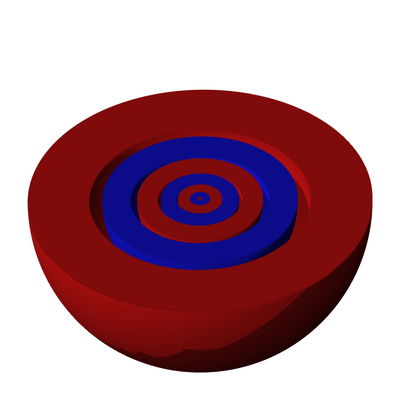
\includegraphics[width=0.5\textwidth]{images/400px-S7M0.png}
    \caption{$7s$轨道的图像}
    \label{fig:s_orbital}
\end{figure}

\subsubsection{$p$轨道}

\begin{equation*}
    Y = \sqrt{\frac{3}{4\pi}} \cos \theta
\end{equation*}

图\ref{fig:p_orbital}展示了$p$轨道的情况

\begin{figure}[h]
    \centering
    
\includegraphics[width=0.5\textwidth]{images/P2y.png}
    \caption{由左而右为2p、3p、4p、5p、6p轨道的立体模型}
    \label{fig:p_orbital}
\end{figure}



\subsubsection{图像的特点}

\begin{enumerate}
    \item $l,m$不同,$n$相同,$Y$相同,$n$与图形无关
    \item $l$不同,$Y$图的形状不同 $l$决定图像的形状
    \item $m$决定$Y$图的伸展方向,决定图像取向
\end{enumerate}

\chapter{多原子电子结构}

\begin{equation*}
	-\frac{\hbar^2}{2m} \nabla_1^2 - \frac{\hbar^2}{2m} \nabla_2^2 - \frac{ze^2}{4\pi\epsilon_0r_1} - \frac{ze^2}{4\pi\epsilon_0r_2} - \frac{ze^2}{4\pi\epsilon_0r_1r_2} \psi = E\psi
\end{equation*}

\section{中心力场法}

如果忽略电子之间的相互特征,将多电子体系转化为单电子体系,并引入一个以原子核为中心的中心力场。这个中心力场可以表现为\textbf{有效核电荷数} $Z^*$。

\subsection{Slater法则}

将电子分层,|1s| , |2s, 2p| , |3s, 3p|, |3d|。屏蔽常数:$\sigma$,同层为0.35, 1s的为0.3,$n - 1$层的为0.85,$n - 2$以上为1。

有效核电荷数

\begin{equation*}
	Z^* = Z - \sum \sigma
\end{equation*}

例如 $\ce{Na}$ $3s^1$,屏蔽常数为

\begin{equation*}
	0.85 \times 8 + 1 \times 2 = 8.8
\end{equation*}

这样$3s^1$轨道的电子能量为

\begin{equation*}
	E = -13.6 \times \frac{11 - 8.8}{9}
\end{equation*}


\section{电子排布的规律}

必须遵循规则:

\begin{enumerate}
	\item Pauli不相容原理
	\item 能量最低原理
	\item Hund规则
\end{enumerate}

\subsection{能级交错}

多电子体系下会出现能级交错的现象。

\begin{equation*}
	ns < np < nd < nf
\end{equation*}

\subsection{钻穿效应和屏蔽效应}

\subsubsection{钻穿效应}

高轨道的s电子在核附近具有较大的密度,被称为\textbf{钻穿效应}。

\subsubsection{屏蔽效应}

低轨道电子对外层轨道电子有较大的屏蔽作用。


\section{分子轨道理论}


\subsection{$\ce{H2+}$氢分子离子}


\begin{equation*}
	\left(-\frac{\hbar^2}{2m} \nabla_1^2 - \frac{\hbar^2}{2m} \nabla_2^2 - \frac{ze^2}{4\pi\epsilon_0r_1} - \frac{ze^2}{4\pi\epsilon_0r_2} \right) \psi = E\psi
\end{equation*}

\subsection{变分法}


选取变分函数$\psi'$ 得到近似解。


最小能量法:

\begin{equation*}
	E = \frac{\int \psi^* \hat{H} \psi \d \tau}{\int \psi^*  \psi \d \tau}
\end{equation*}


\subsection{线性变分法}

\begin{equation*}
	\psi ' = c_1 \psi_1 + c_2 \psi_2 + \dots + c_n \psi_n
\end{equation*}


求最小值需要列方程:


\begin{equation*}
	\frac{\partial E}{\partial c_1} = \frac{\partial E}{\partial c_2} = \cdots = \frac{\partial E}{\partial c_n} = 0
\end{equation*}



\subsubsection{线性变分法处理$\ce{H2+}$氢分子离子}

选取变分函数:


如果$r_a \ll r_b$, 则选取 $\psi_A$

如果$r_a \gg r_b$,则选取$\psi_B$

\begin{equation*}
	\psi = c_A \psi_A + c_B \psi_B
\end{equation*}

\begin{align*}
	\bar{E} & = \frac{\int \psi^* \hat{H} \psi \d \tau}{\int \psi^*  \psi \d \tau}                                                   \\
	        & = \frac{\int (c_A\psi_A + c_B\psi_B) \hat{H} ( c_A\psi_A + c_B\psi_B) \d \tau}{\int (c_A\psi_A + c_B\psi_B)^2 \d \tau} \\
	        & = \frac{\int (c_A\psi_A + c_B\psi_B) \hat{H} ( c_A\psi_A + c_B\psi_B) \d \tau}{\int (c_A\psi_A + c_B\psi_B)^2 \d \tau} \\
\end{align*}


\begin{align*}
	H_{AA} & = \int \psi_A \hat{H} \psi_A \d \tau = \int \psi_B + \hat{H} \psi_B \d \tau \\
	H_{AB} & = \int \psi_A \hat{H} \psi_B \d \tau = \int \psi_B + \hat{H} \psi_A \d \tau \\
	S_{AB} & = \int \psi_A \psi_B \d \tau
\end{align*}



\begin{align*}
	\left( \bar{E} - H_{AA} \right) c_A^2 + \left( 2S_{AB} \bar{E} - 2H_{AB}   \right)c_Ac_B + \left(  \bar{E} - H_{BB} \right)c_B^2 = 0
\end{align*}


能量最低:

分别对$c_A$,$c_B$求导


\begin{align*}
	2 \left(  \bar{E} - H_{AA}  \right)c_A + 2 \left( S_{AB} \bar{E} - H_{AB}  \right)c_B & = 0 \\
	2 \left(  S_{AB}\bar{E} - H_{AB} \right)c_A + 2 \left( \bar{E} - H_{BB}  \right)c_B   & = 0
\end{align*}


\begin{align*}
	\left| \begin{array}{cc}
		       \bar{E} - H_{AA}        & S_{AB} \bar{E} - H_{AB} \\
		       S_{AB} \bar{E} - H_{AB} & \bar{E} - H_{BB}
	       \end{array} \right|
\end{align*}

\begin{align*}
	\bar{E_1} & = \frac{H_{AA} + H_{AB}}{1 + S_{AB}} \\
	\bar{E_2} & = \frac{H_{AA} - H_{AB}}{1 - S_{AB}} \\
\end{align*}

注意,从上式可得:

\begin{equation*}
	c_A = \pm c_B
\end{equation*}

\begin{align*}
	\psi = c_A \psi_A + c_B \psi_B = \begin{cases}
		                                 \psi_1 = c_A(\psi_A + \psi_B) \\
		                                 \psi_2 = c_A(\psi_A - \psi_B)
	                                 \end{cases}
\end{align*}



\subsubsection{重叠积分$S_{AB}$}

\begin{equation*}
	S_{AB} = \int \psi_A \psi_B \d \tau
\end{equation*}

这个积分被称为重叠积分。
\begin{equation*}
	\begin{cases}
		\psi_A = \psi_B \quad S_{AB} = 1 & \mbox{原子核核间距} R \to 0      \\
		S_{AB} = 0                       & \mbox{原子核核间距} R \to \infty \\
		0 < S_{AB} < 1                   & \mbox{成键}                      \\
	\end{cases}
\end{equation*}

\subsubsection{库仑积分$H_{AA}$}

\begin{align*}
	H_{AA} & = \int \psi_A \hat{H} \psi_A \d \tau                                                                                                                                                                                           \\
	       & = \int \psi_A \left( -\frac{\hbar}{2m} \nabla^2 - \frac{ze^2}{4\pi\epsilon_0r_A} - \frac{ze^2}{4\pi\epsilon_0r_B} -  \frac{e^2}{4\pi\epsilon_0R}  \right) \psi_A \d \tau                                                       \\
	       & = \int \psi_A \left( -\frac{\hbar}{2m} \nabla^2 - \frac{ze^2}{4\pi\epsilon_0r_A} \right) \psi_A \d \tau  - \int \psi_A \frac{ze^2}{4\pi\epsilon_0r_B} \psi_A \d \tau + \int \psi_A  \frac{e^2}{4\pi\epsilon_0R} \psi_A \d \tau \\
	       & = E_A - \int \psi_A \frac{ze^2}{4\pi\epsilon_0r_B} \psi_A \d \tau + \int \psi_A  \frac{e^2}{4\pi\epsilon_0R} \psi_A \d \tau                                                                                                    \\
	       & = E_A - J
\end{align*}

其中$E_A$是原子基态的能量,$J$几乎可以抵消。$E_A = E_B \approx H_{AA}$

\subsubsection{交换积分$H_{AB}$}

\begin{align*}
	H_{AB} & = \int \psi_A \hat{H} \psi_B \d \tau                                                                                                                                     \\
	       & = \int \psi_A \left( -\frac{\hbar}{2m} \nabla^2 - \frac{ze^2}{4\pi\epsilon_0r_A} - \frac{ze^2}{4\pi\epsilon_0r_B} -  \frac{e^2}{4\pi\epsilon_0R}  \right) \psi_B \d \tau \\
	       & = \int \psi_A E_B \psi_B \d \tau - \int \psi_A \left(\frac{ze^2}{4\pi\epsilon_0r_B} - \frac{e^2}{4\pi\epsilon_0R} \right) \psi_B \d \tau                                 \\
	       & = E_BS_{AB} +  \left(\frac{ze^2}{4\pi\epsilon_0r_B} - \frac{e^2}{4\pi\epsilon_0R} \right) \int \psi_A \cdot \psi_B \d \tau                                               \\
	       & = E_BS_{AB} + K \left( K < 0 \right)                                                                                                                                     \\
\end{align*}
注意,这里
\begin{equation*}
	H_{AB} - E_BS_{AB} = K
\end{equation*}

$E_BS_{AB}$为负值,同时,$\left(\frac{ze^2}{4\pi\epsilon_0r_B} - \frac{e^2}{4\pi\epsilon_0R} \right)$也为负值,总体来看,$H_{AB}$为负值。这个负值有利于体系总体能量的降低,利于成键。这个积分也被称为键积分。在讨论时为了简化,通常也被称为$\beta$积分。


\begin{align*}
	E_1 & = \frac{H_{AA} + H_{BB}}{1 + S_{AB}}                                               \\
	    & = \frac{H_{AA} + H_{BB}S_{AB}}{1 + S_{AB}} + \frac{H_{BB} - S_{AB}E_B}{1 + S_{AB}} \\
	    & = E_H + \frac{K}{1 + S_{AB}}                                                       \\
	    & = E_H + \mbox{负数}
\end{align*}

$\psi_1 = c_A \left( \psi_A + \psi_B \right) \Rightarrow$ 体系能量比单独的氢原子低,表现为成键轨道。

\begin{align*}
	E_2 & = \frac{H_{AA} - H_{BB}}{1 - S_{AB}}                               \\
	    & = \frac{H_{AA} - H_{AA}S_{AB} + H_{AA}S_{AB} - H_{AB}}{1 - S_{AB}} \\
	    & = H_{AA} + \frac{H_{AA}S_{AB} - H_{AB}}{1 - S_{AB}}                \\
	    & = H_{AA} + \frac{E_AS_{AB} - H_{AB}}{1 - S_{AB}}                   \\
	    & = H_{AA} + \frac{-K}{1 - S_{AB}}                                   \\
	    & = E_H + \mbox{正数}
\end{align*}

$\psi_2 = c_A \left( \psi_A - \psi_B \right) \Rightarrow$ 体系能量比单独的氢原子高,表现为反键轨道。


\section{分子轨道理论和双原子分子结构}

\subsection{分子轨道理论的概念}


分子中的每个电子都可以看作是在各个原子的原子核以及其他电子所组成的平均力场下运动,第$i$个电子的运动状态可以用波函数$\psi_i$来描述。$\psi_i$被称为分子的单电子波函数,又称为分子轨道。分子的总能量为各个电子所处的分子轨道的分子轨道能量之和。


\subsection{分子轨道的形成}

分子轨道$\psi$可以近似地用能级相近的原子轨道线性组合。原子轨道线性组合成分子轨道时,轨道数目不变,轨道能级改变。两个能量相近的原子轨道组合成分子轨道时,能量低于原子轨道能级的称为成键轨道,高于原来两个原子轨道的能级分为反键轨道。

两个分子轨道的形成必须满足以下条件:

\begin{itemize}
	\item 能量相近
	\item 轨道最大重叠
	\item 对称性匹配
\end{itemize}


\subsubsection{能量相近的证明}

设$\phi_a, \phi_b$分别表示两个原子的原子轨道。其中$E_a < E_b$,他们组合成分子轨道。设$H_{aa} = E_a$,$H_{bb} = E_b$,$H_{ab} = \beta$,$S_{ab} = 0$。带入久期行列式,可得:

\begin{equation*}
	(E_a - E)(E_b - E) = \beta^2
\end{equation*}

\begin{align*}
	E_1 & = \frac{1}{2} \left[ (E_a + E_b) - \sqrt{\left(  E_b - E_a \right)^2 + 4\beta^2}  \right] \\
	    & = E_a - U
\end{align*}
\begin{align*}
	E_2 & = \frac{1}{2} \left[ (E_a + E_b) + \sqrt{\left(  E_b - E_a \right)^2 + 4\beta^2}  \right] \\
	    & = E_b + U
\end{align*}

其中

\begin{align*}
	U = \frac{1}{2} \left[ \sqrt{ \left(E_b - E_a\right)^2 + 4\beta^2} - \left(E_b - E_a\right) \right]
\end{align*}

\section{休克尔分子轨道理论(HMO)}

\subsection{适用范围}

只适用于共轭体系,只针对$\pi$电子。

\subsection{$\pi$电子近似}

将所有的化学键看作是原键+$\sigma$键,再加额外的$\pi$电子。


\subsection{线性变分法处理}


\begin{equation*}
	\psi = c_1 \psi_1 + c_2 \psi_2 + c_3 \psi_3 + \cdots + c_n \psi_n
\end{equation*}

久期方程式

\begin{equation*}
	\begin{bmatrix*}
		H_{11} - ES_{11} & H_{12} - ES_{12} & \cdots & H_{1n} - ES_{1n} \\
		H_{21} - ES_{21} & H_{22} - ES_{22} & \cdots & H_{2n} - ES_{2n} \\
		\vdots & \vdots & \ddots & \vdots \\
		H_{n1} - ES_{n1} & H_{n2} - ES_{n2} & \cdots & H_{nn} - ES_{nn}
	\end{bmatrix*} = 0
\end{equation*}

计算过程中做简化处理(表 \ref{tab:simplify}):


\begin{table}[h]
	\centering
	\begin{tabular}{cc}
		库仑积分 & $H_{11} = H_{22} = \alpha$                 \\
		交换积分 & $H_{ij} = H_{ji} = \begin{cases}
				                              \beta & i = j \neq 1    \\
				                              0     & i \neq j \neq 1
			                              \end{cases}$ \\
		重叠积分 & $S_{ij} = \begin{cases}
				                     1 & i = j    \\
				                     0 & i \neq j
			                     \end{cases}$
	\end{tabular}
	\caption{简化处理方法}
	\label{tab:simplify}
\end{table}


\subsection{分子图}

需要计算电荷密度、键级、自由价。

\subsubsection{电荷密度}

电荷密度$\rho_i$第$i$个原子上出现的$\pi$电子数

\begin{equation*}
	\rho_i = \sum_{k} n_k c^2_{ki}
\end{equation*}

\subsubsection{键级}

键级$P_{ij}$表示原子$i$和原子$j$之间成键的强度。

\begin{equation*}
	P_{ij} = \sum_k n_k c_{ki} c_{kj}
\end{equation*}

\subsubsection{自由价}

自由价$F_i$,第$i$个原子剩余成键能力的相对大小。

\begin{equation*}
	F_i = F_{\mathrm{max}} - \sum_i P_{ij}
\end{equation*}


$F_{\mathrm{max}}$的值为$\sqrt{3}$,采用了理论上存在的三次甲基甲烷分子的解。

若要计算三次甲基甲烷的键级,计算久期行列式:

\begin{equation*}
	\begin{vmatrix}
		x & 1 & 1 & 1 \\
		1 & x & 0 & 0 \\
		1 & 0 & x & 0 \\
		1 & 0 & 0 & x \\
	\end{vmatrix}
\end{equation*}


\section{丁二烯的HMO法处理}

丁二烯 \begin{scriptsize}
	\chemfig{=[:30]-[:-30]=[:30]}
\end{scriptsize} 的分子轨道为

\begin{equation*}
	\psi = c_1 \psi_1 + c_2 \psi_2 + c_3 \psi_3 + c_4 \psi_4
\end{equation*}

$\psi_i$表示参加共轭的4个C原子的$p_z$轨道。

久期行列式:

\begin{equation*}
	\begin{vmatrix}
		\alpha - E & \beta      & 0          & 0          \\
		\beta      & \alpha - E & \beta      & 0          \\
		0          & \beta      & \alpha - E & \beta      \\
		0          & 0          & \beta      & \alpha - E \\
	\end{vmatrix}
\end{equation*}

\begin{equation*}
	\begin{vmatrix*}
		x & 1 & 0 & 0 \\
		1 & x & 1 & 0 \\
		0 & 1 & x & 1 \\
		0 & 0 & 1 & x \\
	\end{vmatrix*}
\end{equation*}


\begin{equation*}
	x^4 - 3x^2 + 1 = 0
\end{equation*}

解得

\begin{align*}
	x_1 & = -1.618 \\
	x_2 & = -0.618 \\
	x_3 & = 0.618  \\
	x_4 & = 1.618  \\
\end{align*}

于是

\begin{align*}
	E_1 & = \alpha + 1.618\beta \\
	E_2 & = \alpha + 0.618\beta \\
	E_3 & = \alpha - 0.618\beta \\
	E_4 & = \alpha - 1.618\beta \\
\end{align*}

其中$\alpha = E_{p_z} < 0$,$\beta = c_i \sim c_{i+1} (\mbox{键积分}) < 0$。


\begin{equation*}
	E_1 < E_2 < E_3 < E_4
\end{equation*}

\section{价键理论 杂化轨道理论}

假设$s,p,d$轨道所占的比例分别为$\alpha, \beta, \gamma$,则两个等性杂化轨道间的最大值之间的夹角$\theta$满足

% 杂化轨道

% 正交的

% 归一的

% 杂化是比较解释性的东西(

% 实际去测得话
\begin{equation*}
	\alpha + \beta \cos \theta + \gamma \left(\frac{3}{2}\cos ^2 \theta - \frac{1}{2}\right) = 0
\end{equation*}

对于不等性杂化轨道:

\begin{equation*}
	\sqrt{\alpha_i} \sqrt{\alpha_j} + \sqrt{\beta_i}{\sqrt{\beta_j}} \cos \theta_{ij} + \sqrt{\gamma_i}\sqrt{\gamma_j} \left( \frac{3}{2} \cos ^2 \theta_{ij} - \frac{1}{2}  \right)= 0
\end{equation*}

\section{前线轨道理论和轨道对称守恒原理}

这个部分主要介绍应用量子化学方法研究一般化学反应的动态过程。

\subsection{前线轨道理论}

% Frontier Orbital Theory

\subsection{轨道对称守恒原理}



\end{document}